\section{System Overview}
Human movement is a complex interplay between intentions within the brain and the physical environment. The though to 'walk-forward' triggers and array of intractable optimization  

In the following we will introduce a method for optimal synchronization between a Movement Model and a set of animations given Control Genomes. There are 4 main parts to the system. 
\begin{itemize}
    \item \textbf{Control Genomes} extracted from animations.
    \item \textbf{Movement Model} that generates a movement given Control Genomes.
    \item \textbf{Non destructive} animation smoothing. 
    \item \textbf{Optimization procedure} that fits exposed parameters of all the above systems to minimize the difference between the movement- and animation trajectories.
\end{itemize}
Figure \ref{fig:movement:model} illustrates the definitions and concepts of a movement model.
\begin{figure}
    \centering
    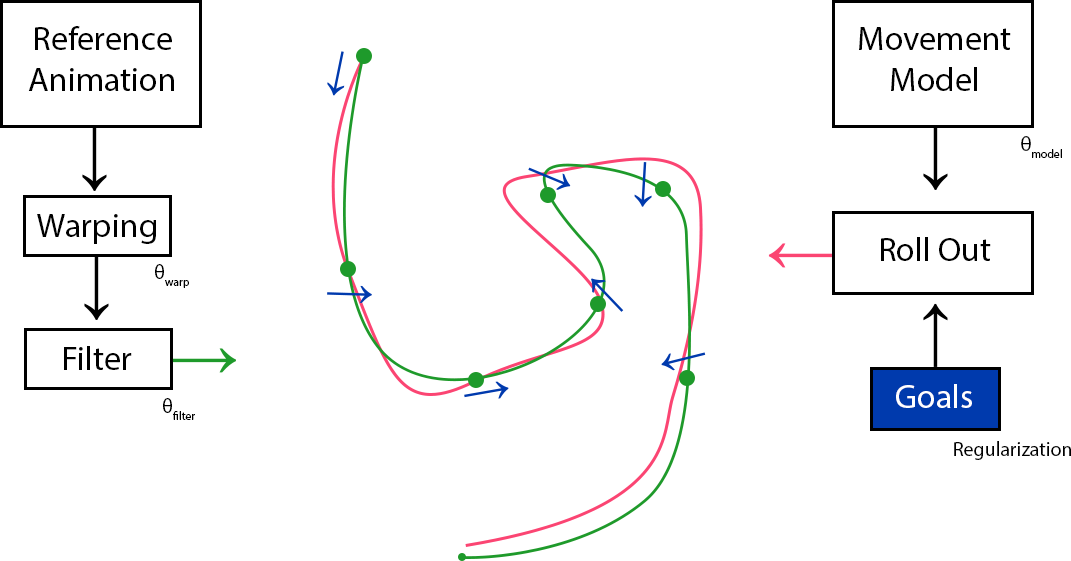
\includegraphics[width=0.75\columnwidth]{img/method-overview.png}
    \caption{Theta values indicate parameters subject to optimization. Goals are fixed to add regularization}.
    label{fig:movement:model}
\end{figure}

\section{Control Genomes}
We define Control Genomes as signals that can generate movement. They are a combination of intentions and enough contextual state to follow the Markov principle. As an example a position, direction and time is a Control Genome for a straight walk. Conversely a straight walk contains a latent Control Genome (position, direction, time). Under this naive framework we quickly realize that multiple straight walks could be associated with a single Control Genome. We further impose the constraint that Control Genomes must disambiguate movement, ie. a unique Control Genome maps to a unique movement. In our simple example we might resolve conflicts by adding a style parameter and assign values such as 'brisk walk' or 'dragging feet' to our Control Genomes. 

Control Genomes can have a direct counter part in the host application such as user input through a game controller or navigational path from an AI system, and therefore can also be viewed as tasks (ie. turn right) that are carried out by the animations. In general we want the Control Genomes to be of minimal size, since in the limit we could have the animation itself as the Control Genome. We say that a genome is in \textit{reduced} and \textit{segmented} form if it contains no repetitions and removal of information would break either the Markov property of the disambiguation constraint. 

\begin{figure}
    \centering
    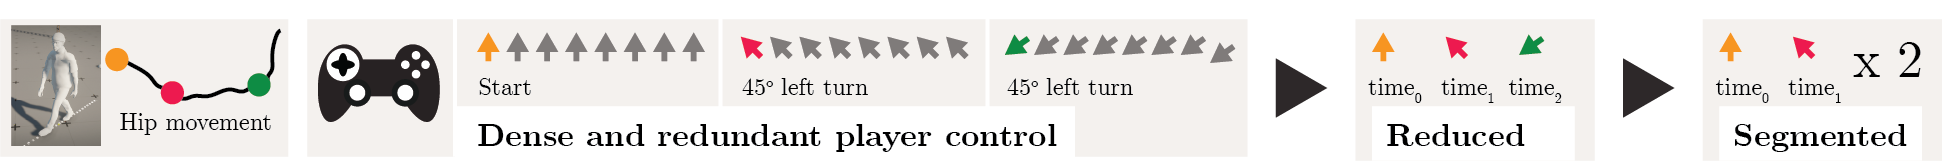
\includegraphics[width=1\columnwidth]{img/controlgenome.png}
    \caption{Control Genome}
    \label{fig:control:genome}
\end{figure}

Figure Fig. \ref{fig:control:genome} shows an example where an animation has been assigned a Control Genome. Each frame is annotated with a 2d-control direction corresponding to stick input from a game controller. A dense and redundant Control Genome contains the entire skeletal animation as well as the annotated directions. The animation has two similar right turns so we get a single segmented Control Genome by splitting the redundant genome in two identical parts. We then trim all unnecessary information from the genome to get the reduced form which only contain a starting position and two direction offset in time. This last step assumes that we are capable of regenerating the animation from the reduced genome using a procedure we will refer to as a \textit{Movement Model}. A [Control Genome, Movement Model]-pair describes an animation exactly when the Movement Model can regenerate the Animation from the Control Genome.  In practice it is not possible to develop accurate generative or predictive models for human movement. So we will allow our animations to undergo non destructive transformation such as smoothing and path adjustment, and only expect our model to regenerate a fraction of the complete signal, such as the trajectory. 

We will now proceed to a formalized description of Control Genomes.

The input to our system is an annotated animation. Let $\anim^{\dimas,\dimaa}_\dimat$ denote $\dimat$ frames of animation of a skeleton with $\dimas$ degrees of freedom, where each frame is given an $\dimaa$-dimensional annotation. We assume the presence of a Retrieve-and-Collapse procedure (automated or manual) that extracts all reduced and segmented Control Genomes present in the animation and for each maintains a pairing to all $k$ corresponding (un-annotated) segments of the source animation. With $i$ and $\dimg$ as the number of and dimensionality of the Control Genomes we have $\genome^g_i\in\reco(\anim^{\dimas,\dimaa}_\dimat)\rightarrow\anim^{\dimas,0}_{\dimae_0}\ldots\anim^{\dimas,0}_{\dimae_k}$ where $\dimae\ll\dimat$ refers to a segment of the full animation and $k$ is the number of segments matched to the $i$'th Control Genome.


We define two parametric projections to a shared $\dimes$-dimensional evaluation space as $\model(\paramm,\genome^{\dimg}) \rightarrow \mathcal{R}^{\dimes}$ and $\edit(\parame,\anim_{\dimae}^{\dimas,0}) \rightarrow \mathcal{R}^{\dimes}$. The evaluation space will usually have a natural counterpart in the application such as the trajectory (position and orientation of character over time).\\
Intuitively $\model$ is a Movement Model capable of generating movement (or more accurately an evaluation space representation) from the Control Genomes. $\edit$ corresponds to the adjustment we allow our animations to undergo, such a smoothing or more advanced manipulation. The optimal parameters for a single Control Genome are found as the minimization of the L2-norm.
\begin{subequations}
\begin{align}
    \gnorm(\paramm,\parame,\genome)&=\sum_{\anim_k\in\genome}{\frac{1}{2}|\model(\paramm,\genome)-\edit(\parame\anim_k)|^2}\\
    \paramm^*,\parame^*&=\min_{\paramm,\parame}{\gnorm(\paramm,\parame,\genome)}
\end{align}
\end{subequations}
When we want constant parameters across the fitting of multiple Control Genomes $\genome_i\in\reco(\genome)$ an additional term is added to the minimization. 
\begin{equation}
    \vec{\paramm^*},\vec{\parame^*}=\min_{\paramm,\parame}{\sum_{\genome_i\in\reco(\genome)}{\gnorm(\paramm^i,\parame^i,\genome_i)}}+VAR(\vec{\paramm},\vec{\parame})
\end{equation}
Where $\vec{\paramm^*},\vec{\parame^*}$ is the full set of parameters and $\paramm^i,\parame^i$ are the parameters fitted to $\genome_i$.

\section{Movement Model}
A movement model describes how an entity moves through space given control input (goals). It consists of internal parameters such as velocities and accelerations. Control input could be a direction of movement supplied by a human using a gamepad, or longer paths supplied by a game engine AI system. We have not seen any formal description of the movement model. Usually some ad hoc newtonian physics concepts are combined with springs and animation curves to control the system \kenny{Thing about generality of your statement, as it stands now you are claiming this is so for all. Hence, can you prove/cite it? Otherwise rephrase so it becomes a more subjective observation from a single context. Like to our knowlege or our observation suggest that.}.

For complex systems such as human beings the movement model has an inherent dichotomy between accuracy and simplicity. Deep Neural Networks are hard to tweak after they have been trained, physical simulations are hard to tune towards artistic expressions while on the other hand a 2-parameter linear model will be too simplistic to capture meaningful details.



In the following we limit \kenny{without loss of generalization} the description to locomotion in the plane. 
\subsection{general frame work}
We parameterize the movement model as 
\begin{equation}
    \label{eq:model:parameterization}
 \model \equiv 
 \left\{ \modes,\,\interpolators \right\}
\end{equation}
where $\modes \equiv \seq{ \mode_1, \ldots, \mode_n}$ is a set of locomotion modes and $\interpolators \equiv \seq{ \interpolator_1, \ldots, \interpolator_m}$ is a set of locomotion mode interpolators that describes the transition between locomotion modes. We use the convention that $\interpolator_j^{a\rightarrow b}$ where $j$ refers to linear index into $\interpolators$ and $a,b$ refers to indices in $\modes$ respectively, ie. $\interpolator^{a\rightarrow b}$ refers to the interpolation between $\mode_a$ and $\mode_b$. A movement model defines the behavior of an actor. 
\begin{subequations}
\begin{align}
    \label{eq:actor:def}
    \actor 
    &\equiv
    \seq{
        \blend, \kine 
        }\\
    \kine
    &\equiv
    \seq{
        \pos, \speed, \move, \dtmove, \facing, \dtfacing 
        }\,,
\end{align}
\end{subequations}
Here $\blend$ are contribution weights for different locomotion modes and $\kine$ encapsulates kinematic properties. $\pos$ and $\speed$ describe position and speed (magnitude of velocity), and movement and facing orientations are quaternions $\move$ and $\facing$ with derivatives $\dtmove$ and $\dtfacing$. Fig. \ref{fig:actor} show a visualization of an $\actor$ in a 3d coordinate system.  
\begin{figure}
    \centering
    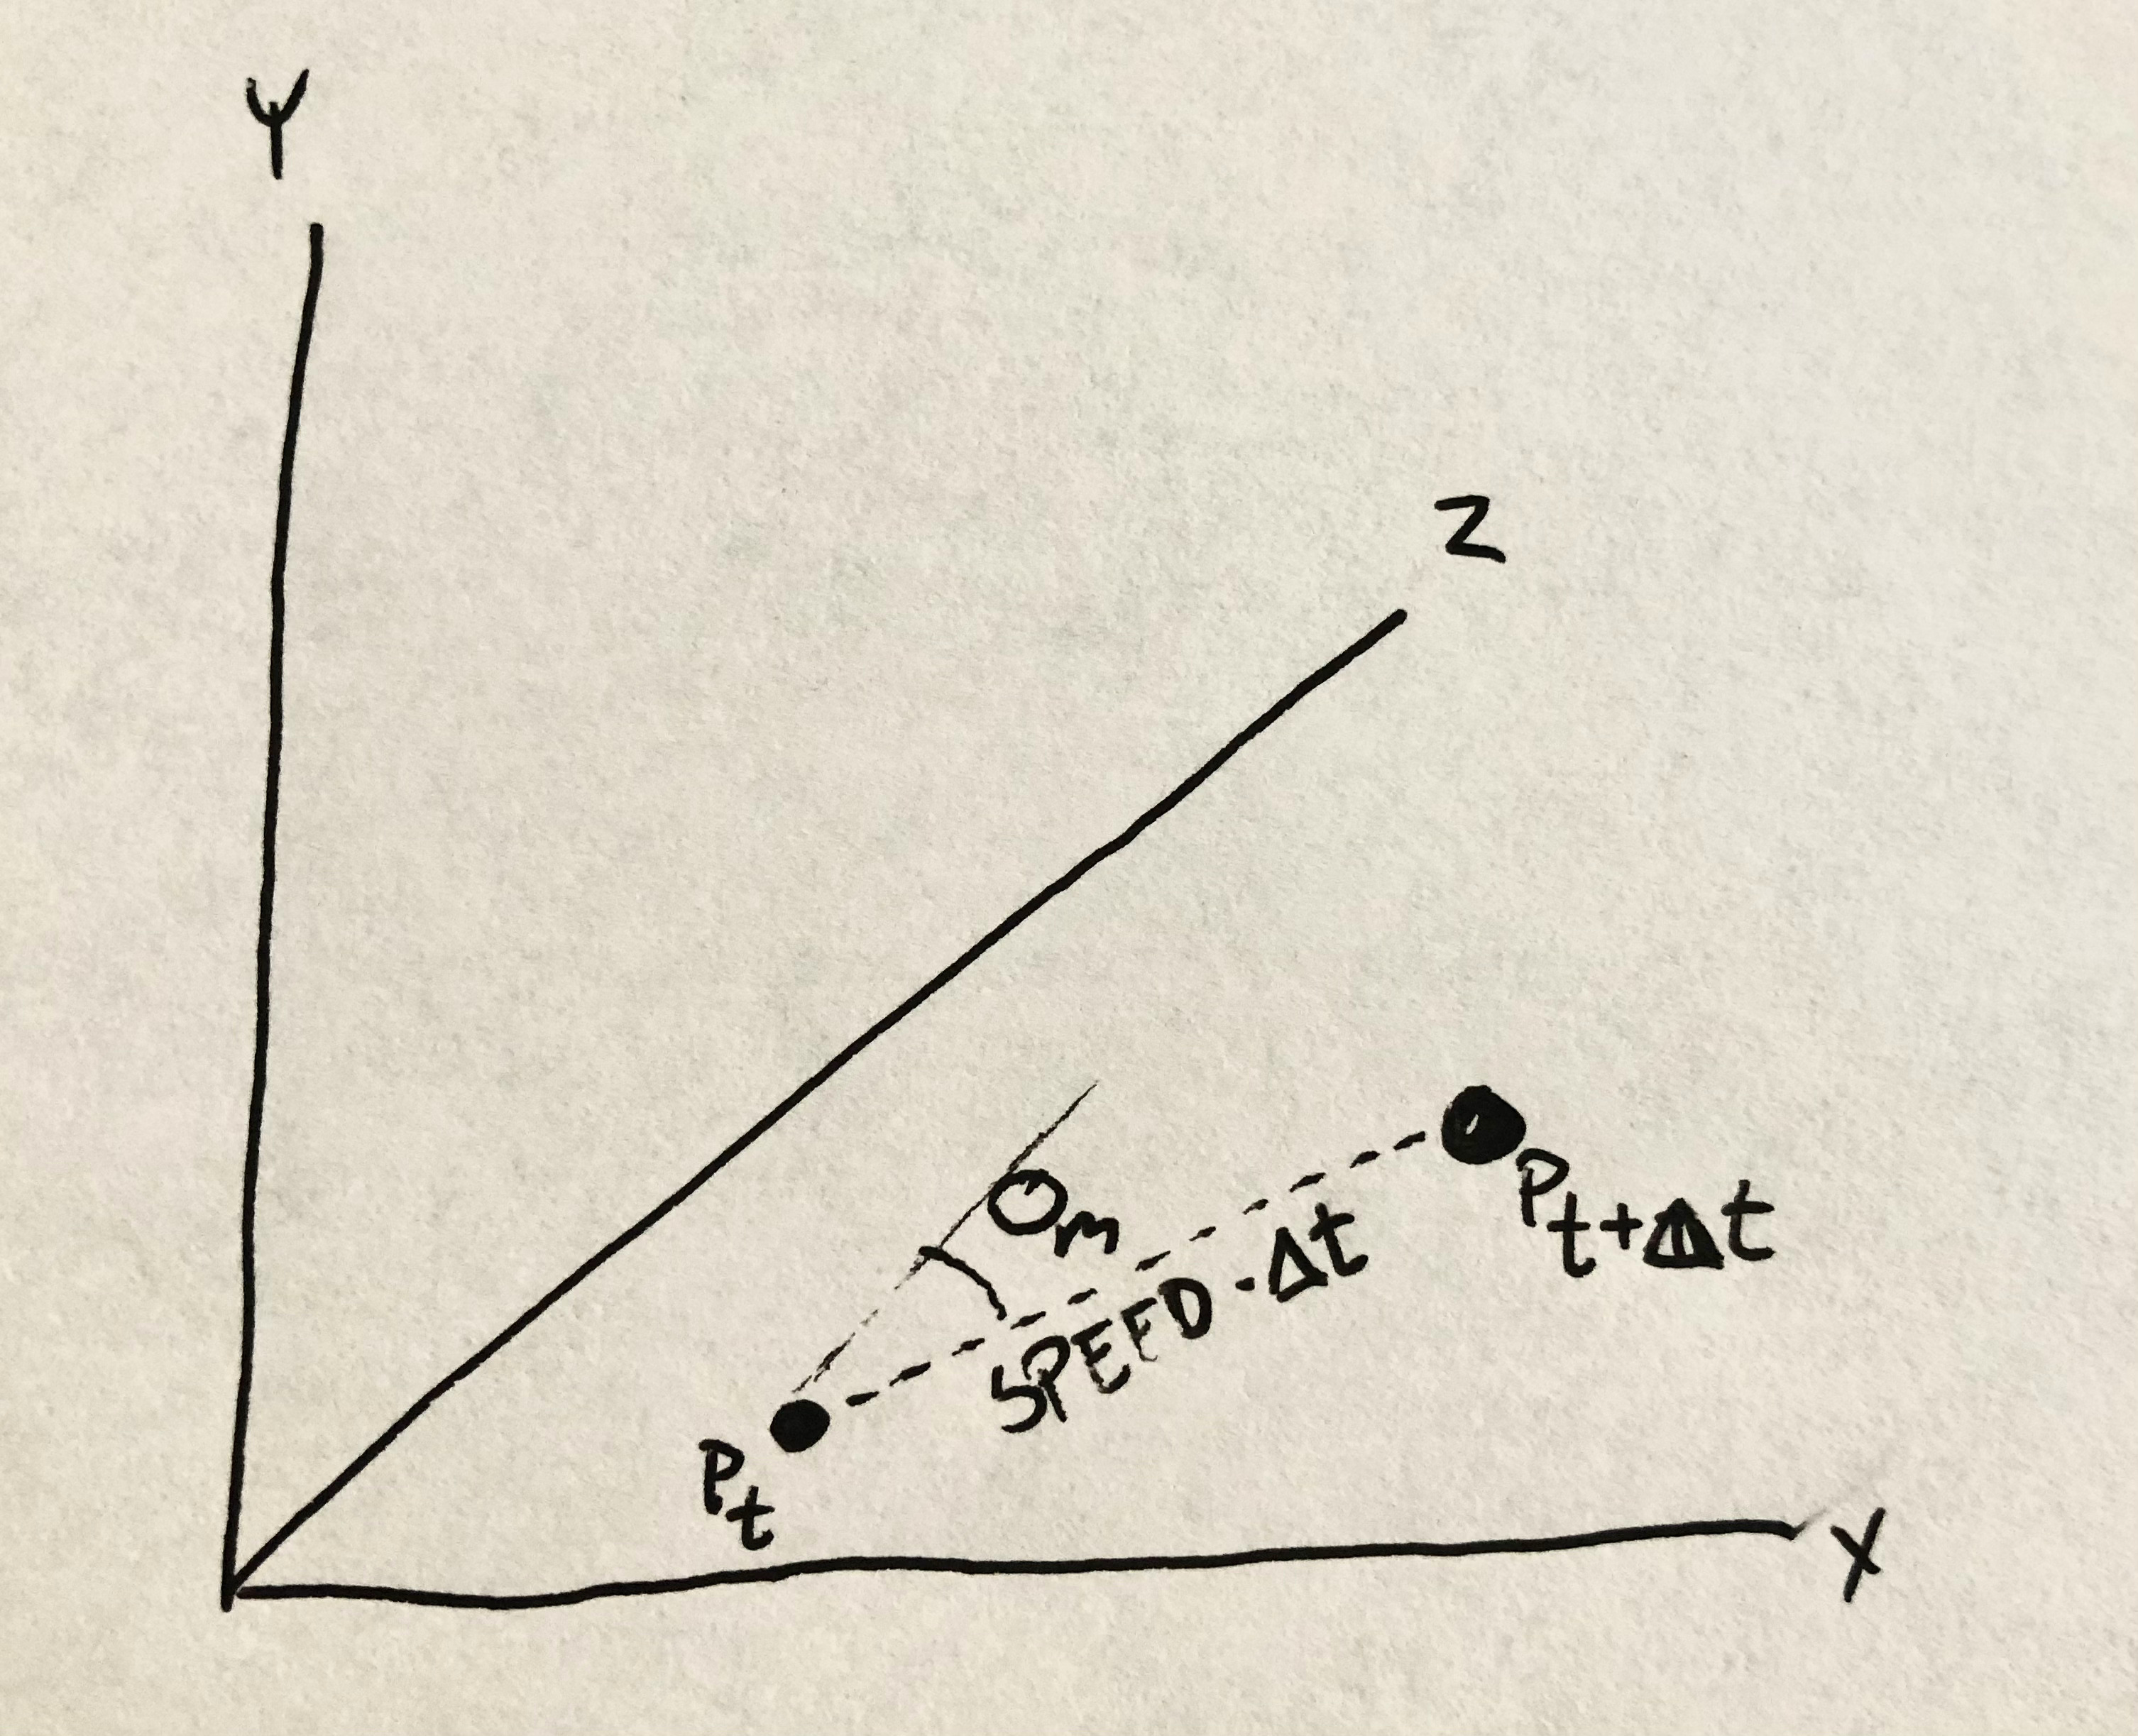
\includegraphics[width=0.75\columnwidth]{img/actor.jpg}
    \caption{Actor. Not showing derivatives and facing orientation}
    \label{fig:actor}
\end{figure}
\kenny{To make this more concrete one can for example think of $\pos$ as the planar 2D position of the character root position in the world and $\ori$ could be the world facing direction of the character given as an angle measure in the 2D world plane.} The contribution weights for different locomotion modes are given by the vector $\blend \equiv \begin{bmatrix}\weight_1 & \ldots & \weight_n \end{bmatrix}^T$ where $\weight_l$ contains the contribution for $l \in \modes$. We impose that $\norm{\blend}^2 = 1$ and remark that usually only a couple of modes will be active as in a transition between walking and running where 
\begin{equation}
    \label{eq:contribusion:weight:example}
    \weight_l \equiv
    \begin{cases}
    0.8 & \text{if $l$ is walking} \\
    0.2 & \text{if $l$ is running} \\
    0 & \text{otherwise}
    \end{cases}\,.
\end{equation}
To describe changes in $\blend$ over time increments $\dt$ each $\interpolator \in \interpolators$ defines a mapping.\kenny{I do not get the notation here, $(\cdot, \cdot)$ is a mapping, maybe it should be written that $\interpolator_{i}^{a,b} : \Re \mapsto \Re^n$ and then one would write $\dweight_{i,b} \leftarrow \interpolator_{i}^{a,b}(\dt)$?} 
\begin{equation}
\dweight_{i,b} \leftarrow (\interpolator_{i}^{a,b},\dt)
\end{equation}
where $\dweight_{i,a}=-\dweight_{i,b}$. \kenny{The sub-index is not really needed? I think you can drop it? The minus sign comes from $\interpolator^{a,b}$ being symmetric opposite to $\interpolator^{b,a}$?}

The locomotion modes and interpolators are activated through high level goals provided by user control input or an AI navigation system. The goals contain no motion planning and should provide only states that we wish to active as fast a possible. Goals are highly context dependent, and for locomotion in the plane we use the following.
\begin{subequations}
\begin{align}
     \goals &\equiv \seq{\mode_g, \kine_g} \label{eq:goals:def} \\
\end{align}
\end{subequations}

where $\mode_g$ and $\kine_g$ is the requested locomotion mode and kinematics respectively. We also use $g$ as subscript for blend weights of the requested locomotion mode.

The sparsity of the goal specification illustrates an inherent uncertainty in character animation, as we are challenged to infer a detailed path of movement through often complex environments given a very limited disambiguation or hints to the desired trajectory \cite{holden.ea16}. We notice that a sampling of the immediate surroundings could potentially be added as part of the goals as in \cite{holden.ea17}. 

A step of the actor state can be described by $\actor_{t+1} = step_{\actor}(\actor, \modes, \interpolators, \goals)$ and split into two separate functions to make the update process clearer.
\begin{subequations}
\begin{align}
    \blend_{t+1} &\leftarrow \sfunc_{\blend}( \blend_{t}, \interpolators, \mode_g, \dt) \label{eq:step:interpolators}\\
    \delspeed, \delmove, \delfacing &\leftarrow  \sfunc_{\kine}(\blend_t, \kine_{t},  \modes, \kine_{g}, \dt )\label{eq:step:modes}
\end{align}
\end{subequations}
Intuitively $\sfunc_{\blend}$ moves $\blend$ towards $w_g=1$ and $w_{i\neq{g}}=0$ using the combined interpolation rules in $\interpolators$. Since multiple interpolators can be active at the same time, we define the contribution $\weighti_k$ of $\interpolator_k$ as the weight of the locomotion mode $k$ relative to the weight of all locomotion modes we are interpolating out of. 
\begin{equation}
\theta_{k}=\dfrac{\weight_k}{\sum{\weight_n}},
\quad \forall k, n \neq g \,.
\end{equation}
The combined effect of multiple active interpolators on $\weight_g$ follows.
\begin{equation}
\dweight_g = \sum \weighti_k \dweight_{i,k} \,,
\quad \forall k \neq g \,.
\end{equation}
We set $\weight_{g,t+1}=\weight_{g,t}+\dweight_g$ and need to maintain both $||\blend||^2=1$ and the distribution of the locomotion modes we are transitioning away from. Both is achieved by.

\begin{equation}
\weight_k = \theta_k \, (1-\weight_g)  
\end{equation}
As en example, the table shows a transition to locomotion mode $\mode_g$ starting with $[\mode_i,\mode_j]$ as active. The transition uses two interpolators $[\interpolator^{i,g},\interpolator^{j,g}]$ in the timespan $0<=t<=2$.
\begin{center}
 \begin{tabular}{||c c c c||} 
 \hline
 t & $\weight_i$ & $\weight_j$ & $\weight_g$  \\ [0.5pt] 
 \hline\hline
 0.0 & 0.4 & 0.6 & 0.0 \\ 
 \hline
 1.0 & 0.2 & 0.3$\bar{3}$ & 0.5 \\
 \hline
 2.0  & 0.0 & 0.0 & 1.0 \\
 \hline
\end{tabular}
\end{center}

\magnus{
\begin{center}
 \begin{tabular}{c c} 
 $(\interpolator^{i,g},1.0)=$ & 0.65\\ 
 $(\interpolator^{j,g},1.0)=$ & 0.4\\ 
\end{tabular}
\end{center}
}

To evaluate $\sfunc_{\kine}$ we notice that each $\mode\in\modes$ should provide update routine $\delspeed_t, \delmove_t \delfacing_t \leftarrow \efunc(\mode, \actor_t,\goals_t)$ which are then weighted.
\begin{subequations}

\begin{align}
\delspeed_t, \delmove_t \delfacing_t &\leftarrow \sum_{k=1}^{n}\weight_k \efunc(\mode_{k},\actor,\goals)\\
\end{align}
\end{subequations}
And used to integrate $\kine$.

\begin{subequations}
\begin{align}
    \pos_{t+\Delta t} &\leftarrow \pos_t + \int_{t}^{t+\Delta t} \dtpos_t\,dt \,, \label{eq:time:int:pos}\\
    \ori_{t+\Delta t} &\leftarrow \ori_t + \int_{t}^{t+\Delta t} \dtori_t\,dt\,, \label{eq:time:int:orientation}\\
    \kine_{t+\dt} &\leftarrow (\kine_t, \pos_{t+\Delta t}, \ori_{t+\Delta t})
\end{align}
\end{subequations}
A simple forward Euler scheme suffices is our choice due to simplicity and performance.

A trajectory is generated by inputting a time series of goals to a Movement model which is then unrolled recursively over time.
\begin{equation}
    [\kine_0 \ldots \kine_t] \leftarrow Unroll(\model,[\goals_{0} \dots \goals{t}])
\end{equation}
For analysis we are not interested in the full $\kine$ state, but only the position and facing orientation in $(\pos, \ori_f)$ which are both available in $\kine$. 
\\\\
To achieve expressive modes we will compose each individual locomotion mode from movement templates. Each template should be easy to understand and modify. Consider the example of running. This would consist on 1 movement template for general locomotion, but then sharp turn might have such a significant strategy that we need more modeling flexibility within the locomotion mode. We would then include a 'sharp turn strategy' as a movement template. Another approach would be to separate running into two distinct locomotion modes (running vs. sharp turn running). However, this would complicate controls, since the user would need to specifically request running or sharp-turn-running. 


\subsection{Trajectory Filter}
An animation is a time series of bone positions and rotations ordered in a hierarchy or skeleton and changing over time.  
\begin{subequations}
\begin{align}    
    \skeleton=&[(\vec{v}_{0,0},\quat{q}_{0,0}), \dots, (\vec{v}_{0,b},\quat{q}_{0,b})]\\
        &\dots \\
            &[(\vec{v}_{t,0},\quat{q}_{t,0}), \dots, (\vec{v}_{t,b},\quat{q}_{t,b})]
\end{align}    
\end{subequations}
A filter transforms an animation to a single 'track'. 
\begin{equation}
    [\vec{v}_0,\quat{q}_0 \dots \vec{v}_t,\quat{q}_t] \leftarrow \ffunc(\skeleton)
\end{equation}
A trajectory is a measure of the overall movement described by the animation. Various heuristics exist to extract trajectories from animations such as projection of hip position to movement plane, plane normal to triangulation between hips and shoulders, estimation of center of mass etc. Each method can be viewed as a filter on the full animation.\\\\
To determine whether such a filter produces a good trajectory, we need a measure of success. This is often not made explicit. We have.
\begin{itemize}
    \item Reproducible by some simpler model
    \item Minimize divergence from full skeleton 
\end{itemize}
The first measure is the one most commonly addressed, as it is common to use a simple spline curve as control input to a generative animation system. Now since the requirement is that the spline matches the trajectory of the source animation, we could for instance apply smoothing to the projected hips to achieve a signal that more resembles a perfect spline, that the raw motion of the hips would.\\
The seconds measure implies that we are not free to apply any filtering since the trajectory is used to position a character. Visual coherence such as positioning and pose blending brakes down if the trajectory is modified without constraint.\\
Mathematically we can formulate the measures by.
\begin{equation}
    \epsilon_a=\min_{\theta_f,\theta_m,{\goals_{0\dots{t}}}}\sum{||\ffunc(\theta_f,\skeleton)-\ufunc(\model(\theta),\goals_{0\dots{t}})||^2 }
\end{equation}
\magnus{How do we formulate second meassue ? If two frame are similar in source animation. They should remain similar when trajectory is used as reference instead of hips. Enforces consistency in way trajectory is estimated relative to similarity expressed by animation it self.}



success criteria. How good does it describe position of character ? How easy is it to replicate ?


\subsection{Optimization}
We chose auto differentiation as our optimization framework. \magnus{motive ?}. 
\\\\
Now, this requires the all our building blocks are differentiable across the parameter space.
\\\\ 
Our problem is ill posed. If we allow any type of $\goals$ (control signal) we could make any type of movement model fit our animations. We want controls to correspond to realistic user input. So we do a pre-pass over our animation  with a heuristic that computes plausible goals at certain key frames. We maintain goals between key frames.
\\

We also do a heuristic pre-pass over the animation to estimate locomotion mode at each goal keyframe.
\\
Finally we apply a heuristic to identify where movement templates should be applied.
\\
We use \magnus{term from reinforcement learning. Start with easy examples, progress to harder}. We fit all segments in the animation with individual  locomotion modes (including movement templates).
Now we have two further steps.
\begin{itemize}
    \item \textbf{Align} fitted locomotion modes. 
    \item \textbf{Collapse or discard} locomotion modes.
\end{itemize}


Let's go through an example of the optimization. Imagine we have 4 steps, in an animation containing 2 locomotion model. And goals key framed at 1 and 3. For the sake of simplicity our goals only define a direction in the plane instead of full kinematics state $\kine$.
\begin{subequations}
\begin{align}
    \goals_0&={0,[0,1]}\\
    \goals_1&=\goals_0\\
    \goals_2&={1,[1,0]}\\
    \goals_3&=\goals_2
\end{align}
\end{subequations}
So we are requesting locomotion mode 0 at the first two keyframes, and want to move along the y-axis in the plane. The last two requests locomotion mode 1 and moves along the x-axis.
\\
Since our goals are fixed we can precompute $[\weight_1 \ldots \weight_4]$ using $\sfunc_{\omega}$.
\\
Then we unroll the movement model.
\begin{subequations}
\begin{align}
    \kine_1 &=\sfunc_{\kine}(\blend_1, \kine_0, \modes, \kine_{g,1}, \dt )\\
    \kine_2 &=\sfunc_{\kine}(\blend_2, \kine_1, \modes, \kine_{g,2}, \dt )\\
    \kine_3 &=\sfunc_{\kine}(\blend_3, \kine_2, \modes, \kine_{g,3}, \dt )\\
    \kine_4 &=\sfunc_{\kine}(\blend_4, \kine_3, \modes, \kine_{g,4}, \dt )\\
\end{align}
\end{subequations}
\\\\
Use warp and filter to extract 4 trajectory points. Define optimization.

\subsection{Plane Locomotion}
Examine some concrete models. What parameters do they have ? 
\\\\
 Movement templates: Turn strategy and maybe vaulting strategy as an extension.

\subsection{regularization REST OF TEXT IS JUNK}

\magnus{A movement model outputs a control signal. If we add more and more details to this signal, in the end we will output the entire animation. Some system output a path augmented with footsteps. If we augment with more details we move towards full synthesis by movement model. Balance between descriptive and understandable}

All 

Define an animation.
Define a trajectory extraction
Purpose of trajectory is dual . Stay consistent. Similar animation should have similar trajectories. Re replicatable by movement model. 
Define realization of movement model. 
Define optimization.


How do we fit a movement model ? What is the optimization criterion ?

\subsection{Plane locomotion}

This is the general framework. Now we define locomotion modes and transitions. An actual implementation of the movement model

For $\sfunc_{\vec \omega}$ to keep the transitions defined in $\Delta{t}_c$ updates, each $\interpolator\in\interpolators$ should define a mapping $\Delta{t} \rightarrow \Delta \interp$ which also describes the duration of that transition since $\interp=1$ implies a completed interpolation. Each individual $t$ can be modeled uniquely or in a unified approach, using animator supplied curves, Sigmoids, linear interpolation or even a neural network to capture more subtleties in the transitions. In the case of transitions that are interrupted, we simply freeze existing transitions, and perform the incoming transition as a weighted combination of multiple transitions as shown in Figure \ref{fig:frozen-transition}. 
\begin{figure}
    \centering
    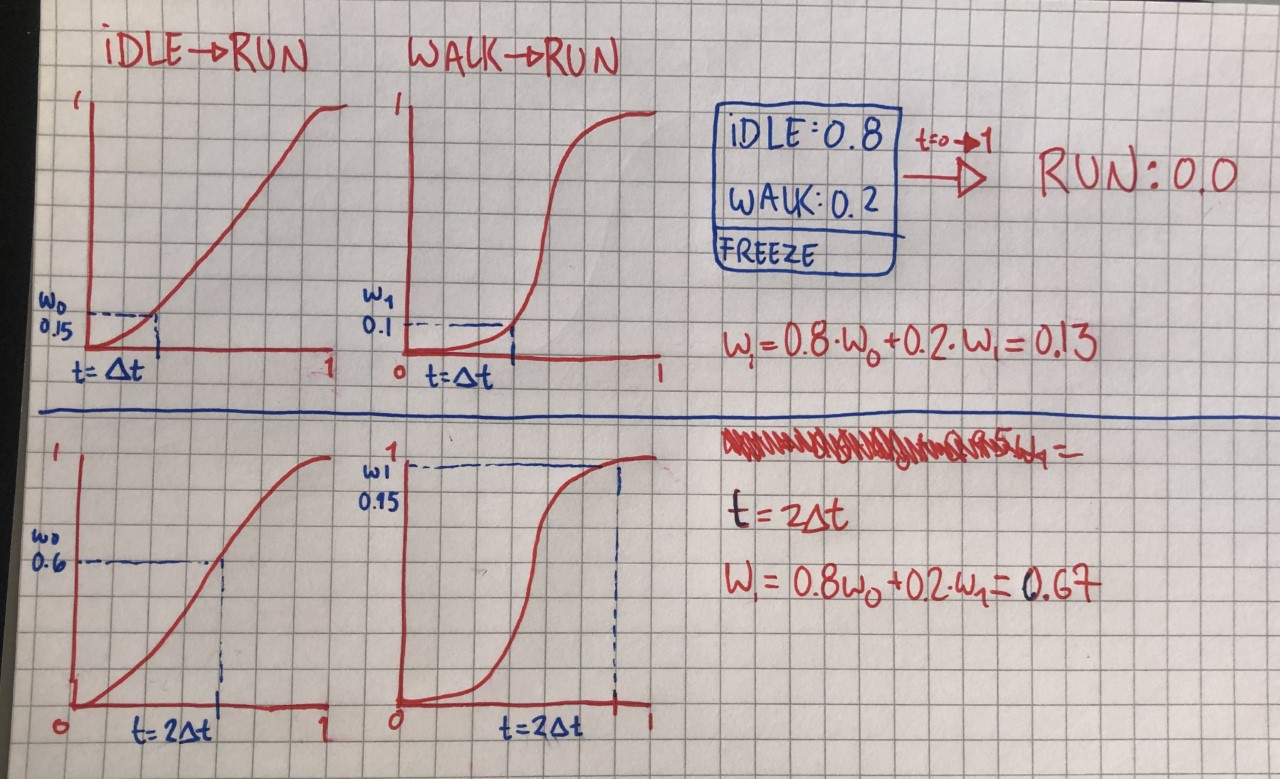
\includegraphics[width=0.75\columnwidth]{img/frozen-transitions}
    \caption{Frozen transition \kenny{Describe the take home message that reader should get from the figure}.}
  \label{fig:frozen-transition}
\end{figure}

By freezing and combining transitions in the case of interruptions, we are effectively approximating missing areas of the locomotion mode manifold by interpolations. This could be avoided by expanding $\interpolators$ to also contain transitions between combination of locomotion mode, or by expanding $\modes$ for a wider sampling of the manifold.

 using $\Delta{t}$. As before the update routines can be arbitrarily complex, which is natural given the idiosyncrasy of human movement. As such our choice of expressiveness in these function are imposing limits on the types of locomotion we are able to model. We use a simple yet expressive approach common to game development.   

velocity, velocity damper function, movement spring constant, orientation spring constant

velocity magnitude depends on the amount angular rotation. Slower when curving
move from current velocity to requested velocity is handled by spring.
move from orientation to requested orientation handled by soring.
Parameters are velocity, velocity damper function, velocity spring constant, orientation spring constant.


Notice that the formulation for $D$ is generic. In production a mapping between the generic movement model and a more context specific model would usually be needed. 

\subsection{missing}
Add animator constraint to model ? Example is 180. We dont start moving backwards immediately. First we rotate 90 degrees on the spot and then we start a 90 degree run to idle movement
Handle this by setting limits on rotation relative to forward movement ? Better to have a locomotion mode where velocity magnitude is 0 when facing relative to direction i < threshold.

Clear description of entire parameter set

Show very clear example. Pseudo code with idle and walk state. 



\section{Basic terminology}
Define animation database as $\mathcal{D}$

Define Movement model

Define Animation warping.


\section{Animation Warping}
We need a warping system that preserves ground truth. And some linear metric for divergence than can be scaled up from 0.


\section{Optimization Procedure}
We need some regularization to ill posed problem
\subsection{Primary movement modes}
Idea: Identify areas in the animations with cyclic movement for some duration. Cluster these segments into buckets with some threshold. We now have the velocity and number of main movement modes.
\subsection{Sparse user input}
If we allow extremely high frequency changes in the user input a wide variety of movement model configurations could follow the animation trajectory. We distribute sparse changes in user input over the animations, ie. few keypoints where we identify changes in the user input.


